\documentclass[11pt,a4paper]{article}
\usepackage[utf8]{inputenc}
\usepackage[T1]{fontenc}
\usepackage[french]{babel}
\usepackage{amsmath,amssymb}
\usepackage{graphicx}
\usepackage{geometry}
\geometry{margin=2.5cm}

\title{La spirale de l'inverse du temps de Philippôt}
\author{Philippe Thomas Savard}
\date{}

\begin{document}

\maketitle

\section*{La spirale de l'inverse du temps de Philippôt :}

\subsection*{1.0}
Le présent document est rédigé avec une liberté de conscience complète et ne bénéficie d'aucun financement n'y d'avantage de quelconque nature pour sa rédaction et sa création.

Ce document est le fruit du travail d'un simple ouvrier qui n'a pas de formation du point de vue des mathématiques. Il est conçu avec un intérêt certain pour cette discipline et par plaisir intellectuelle profond avec le sujet.

\begin{figure}[h]
    \centering
    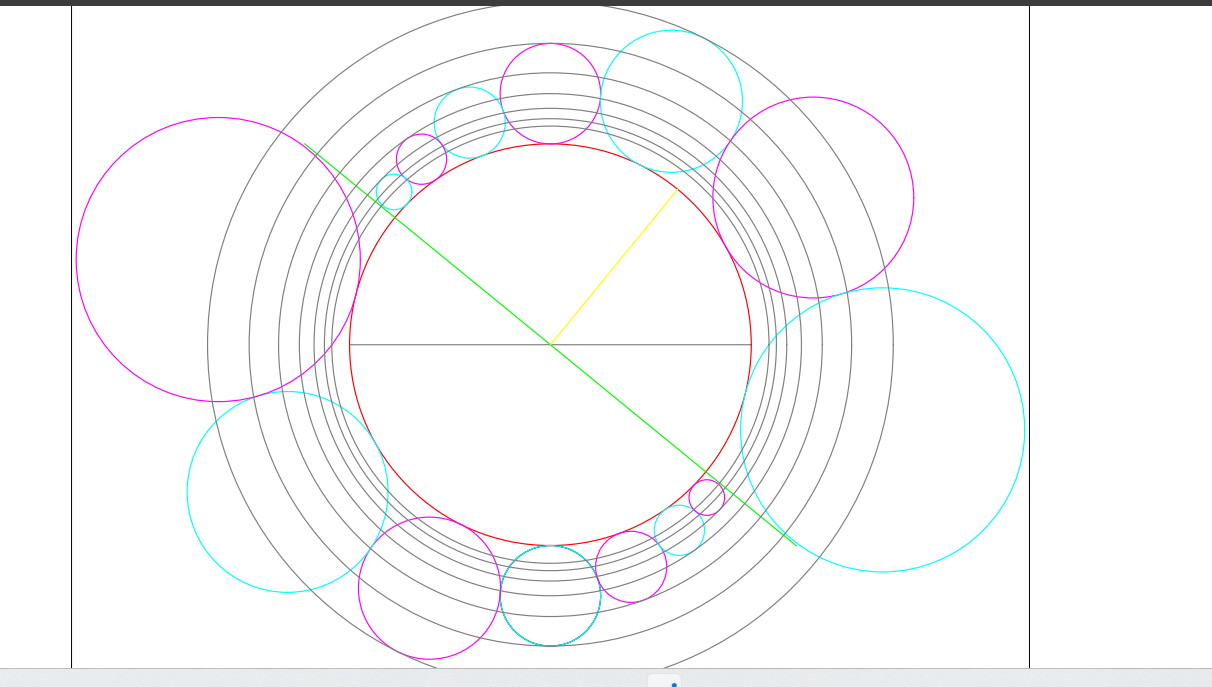
\includegraphics[width=0.8\textwidth]{spirale_inverse_temps.png}
    \caption{Illustration : spirale\_inverse\_temps}
\end{figure}

\subsection*{2.0 Introduction :}
La spirale de l'inverse du temps de Philippôt est un schéma géométrique qui inclut 15 disques tangents les uns les autres. Pour décrire de manière plus complexe il s'agit d'un disque de $2\pi=2\sqrt{10}$ de rayon de 1 sur lequel il se trouve 2 fois une série de 7 disques tangents au disque de de $2\sqrt{10}.$ Les sept disques tangents sont les sept jours de la semaine du dimanche au lundi et du lundi au dimanche le disque du centre est considéré comme étant le lundi à venir au bout de 7 jours les sept disques qui sont tangent a se disque représentant le disque de lundi prochain sont donc situé sur le disque du futur.

Les aires de ces disques suivent la progression de la méthode de Philippôt et des termes de rapports $\frac{1}{k}=\frac{1}{2}$ :
\[ 1-\left(\frac{\sqrt{10}-\frac{(\sqrt{1.6})^{-3}}{10}}{\sqrt{10}}\times\frac{1}{2}\right)=\frac{1}{128}=1-\left(\frac{\sqrt{10}-(Aire~du~disque)}{\sqrt{10}}\right)=Fractions~de~la~methode. \]

Les aires des 8 disques :
\begin{itemize}
    \item $A1=\frac{\sqrt{1.6}^{-3}}{10}\times\frac{1}{2}$
    \item $A2=\frac{\sqrt{1.6}^{-3}}{10}$
    \item $A3=2\times\frac{\sqrt{1.6}^{-3}}{10}$
    \item $AA=4\times\frac{\sqrt{1.6}^{-3}}{10}$
    \item $A5=8\times\frac{\sqrt{1.6}^{-3}}{10}$
    \item $A6=16\frac{\sqrt{1.6}^{-3}}{10}$
    \item $A7=32\times\frac{\sqrt{1.6}^{-3}}{10}$
    \item $A8=64\times\frac{\sqrt{1.6}^{-3}}{10}$
\end{itemize}

La valeur de la constante de l'inverse du temps $=\sqrt{1.6}^{3} = 2.023857703$

Les sept disques de la droite vers la gauche pour la série de disques du haut vont du dimanche rayon $=\sqrt{1/2}$ samedi- $=\frac{1}{2}$ vendredi $\sqrt{1/8}$ jeudi $=1/4$ mercredi $=\sqrt{1/32}$ mardi $=\frac{1}{8}$ et lundi $\sqrt{1/128}$ le disque du centre ayant un rayon de 1. La spirale de l'inverse du temps pour l'auteur est une $9^{ieme}$ solutions au problème d'Apollonius et le problème des contacts.

En effet l'auteur affirme que les sept disques sont également répartit sur $Pi(\pi)$ et que cette représentation permet une autre solution au problème des contacts d'Apollonius.

Comme nous avons pu l'observer dans l'exemple précédent sur les aires des disques qui sont en quelque sorte elles-mêmes en lien avec les valeurs fractionnaires $\frac{1}{k}=\frac{1}{2}$ de la méthode de Philippôt. Sont grandement influencé par la constante de l'inverse du temps.

Cette constante de l'inverse du temps est proposé par l'auteur Philippe Thomas Savard dans l'univers est au carré comme étant la valeur représentée de la valeur de la de la terre 40960 Km qui correspond au volume du diamètre de la terre $\times10^{-2}$.

Valeur de la constante de l'inverse du temps:
\[ \sqrt{circonference~de~la~terre}=\sqrt{40960}Km=\sqrt{diametre~de~la~terre}^{3}\times10^{-12}km \rightarrow \sqrt{160000000}^{3}\times10^{-12}km \]
\[ \sqrt{40960}\times10^{-2}km=2.023857703 \]

C'est sur cette superficie que l'être humain fait l'unique travail auquel il a se pencher savoir 1 litre eau $=10^{79}$ bits unité d'information sur un diamètre d'environ 12000 kilomètres pour un volume égale à la de sa circonférence il accomplie son travail savoir 1litre eau $10^{79}bits$.

La constante de l'inverse du temps $\sqrt{1.6}^{3}=2.023857703$ est une constante qui sert a déterminer un ordre prédéterminé comme $\frac{1}{8.1}=0.1234567901$ .

Ces nombres 0.1234567901 sont en soit lorsque l'on fait allusion a cette constante un ordre d'une séquence donné comme pour 0.1234567901 un ordre s'une séquence chronologique dans l'ordre croissant.

Comme pour cette expression la constante de l'inverse du temps sert a remettre dans un ordre autre que celui pré établie.
\[ Ex:\frac{6.48}{\sqrt{10}}=2.049155924\rightarrow\frac{\sqrt{1.6}^{3}}{2.049155924}=0.987654321 \]
\[ \frac{(0.512\times\sqrt{10})}{6.48/\sqrt{10}}=0.7901234567901 \]

Cette manière de décomposé une séquence d'événement ou d'actes dans un ensemble permet selon l'auteur a l'aide de la méthode de Cantor qui est cependant modifié de déterminer que les nombres premiers et composés sont uniformément répartie entre une surface de $1\times1$ carré par exemple pour les nombres composés et les nombres premiers sur le diamètre sont présents en même quantité.

L'approche que l'auteur emplois est toute fois différente et se matérialise à l'aide d'une droite unique qui est le diamètre où sont placé les nombres premiers qui sont en même quantité que les nombres composés sur la surface.

Cette droite inclut les nombres premiers positif et les nombres premiers négatifs. Elle se constitue à partir de l'affirmation suivante $100\%\times0=0$ les valeurs les plus près de zéro en analyse non standard représente la valeur de l'infini.

Mais pour l'auteur des valeurs comme 101\%, 102\%, 103.\%... de zéro forme à chacun un zéro plus grand mais toujours égale a zéro ces valeur égale à zéro mais plus grande par exemple si on les prend pour des espace vide 0 toujours plus grand par conséquent égale à zéro mais sont en soit les plus près de zéros et représente l'infini.

Les nombres premiers comme expliqué dans d'autre chapitres sont pour l'auteur n'a qu'a penser aux comparaisons asymétriques chaotiques et asymétriques ordonnées ou les nombres premiers démontre bien leur lien du au cardinal des infinis et a l'ordinal dans le cas des comparaisons chaotiques et ordonnées que les nombres premiers sont tous des infinis chacun. Donc la droite des pourcentages de zéros pour les valeurs paires correspondent à un nombre premier positif et les valeurs impaire sa un nombres premiers négatifs.

Ex:
\begin{itemize}
    \item $100\%\times0=0$
    \item $101\%\times0=-2$
    \item $102\%\times0=2$
    \item $103\%\times0=-3$
    \item $104\%\times0=3$
    \item $105\%\times0=-5$
    \item $107\%\times0=5..$
\end{itemize}

Se faisant la méthode s'applique a des valeurs toujours en lien avec la constante de l'inverse du temps.
\[ (\frac{\sqrt{12.34567901}}{\frac{10}{9}})^{2}=10 \text{ (1,0)} \]
pour initier la démarche qui tente d'impliquer les mêmes règles que Cantor qui pour démontrer que sur un carré de $1\times1$ il y a autant de point sur le diamètre que sur la surface de ce carré il décompose des nombres périodiques pour les reformés et démontré la méthode il est toujours préférable de toujours se tenir à côté de 9 comme 0.22222... Et d'interchanger les donné pour former de couple qui deviennent à l'aide de la méthode des points sur la surface et le diamètre?

Suite de l'exemple:
\[ (\frac{\sqrt{23.456790123}}{\frac{10}{9}})^{2}=19(1,9) \]
\[ (\frac{\sqrt{34.56790123}}{\frac{10}{9}})^{2}=28(2,8) \]
\[ \frac{\sqrt{45.679012345}}{10/9}=37(3,7)... \]
est ainsi fait pour un cycle

Autre exemple ensuite se serait 46, 55, 64, 73, 82, 91 et un tour complet
\[ \frac{1.234567901}{2}=0.6172839506 \]

\begin{enumerate}
    \item $(\frac{\sqrt{0.6172839506}}{\frac{10}{9}})^{2}=0.5(0,5)$
    \item $(\frac{\sqrt{0.172839506}}{\frac{10}{9}})^{2}=0.14(1,4)ou(0,14)$
    \item $(\frac{\sqrt{0.72839506}}{\frac{10}{9}})^{2}=0.59(5,9)$
    \item $(\frac{\sqrt{0.2839506}}{\frac{10}{9}})^{2}=0.23(2,3)$
    \item $(\frac{\sqrt{0.839506}}{\frac{10}{9}})^{2}=0.68(6,8)$
    \item $(\frac{\sqrt{0.39506}}{\frac{10}{9}})^{2}=0.32(3,2)...$
\end{enumerate}

(5,0), (5,9), (6,8)...
(1,4), (2,3), (3,2)...

Ces exemples démontrent bien ce a quoi la constante de l'inverse du temps peut être utilisé et ces utilité mathématiques.

\end{document}